\appendixsection{Оценка ресурсов для RSA-2048}

\subsection*{Введение}

Сколько квантовых ресурсов требуется для факторизации 2048-битного RSA-числа? В
этом разделе мы сосредотачиваемся на конкретных квантовых ресурсах, необходимых
для факторизации 2048-битного RSA-числа на основе алгоритма SQIF.
Рассматриваемые квантовые ресурсы в основном включают количество физических
кубитов и глубину схемы QAOA с одним слоем. Обычно квантовые схемы не могут
быть непосредственно выполнены на квантовых вычислительных устройствах,
поскольку при их разработке не учитываются особенности связности кубитов или
топологии реальных физических систем. Процесс выполнения часто требует
дополнительных квантовых ресурсов, таких как вспомогательные (ancilla) кубиты и
увеличение глубины схемы. Мы обсуждаем необходимые квантовые ресурсы для
факторизации реальных RSA-чисел в терминах трёх типов топологий: полной
графовой топологии ($K_n$), двумерной решётки (2DSL) и одномерной цепочки
(LNN). Мы демонстрируем с использованием конкретных схем, что процесс внедрения
(embedding) не требует дополнительных кубитов. Более того, глубина схемы QAOA с
одним слоем линейно зависит от размерности $n$ квантовой системы для всех трёх
топологий. Таким образом, для факторизации целых чисел с использованием
алгоритма SQIF мы потребляем сублинейное количество квантовых ресурсов. В
качестве примера рассмотрим RSA-2048. Необходимое количество кубитов
оценивается как $n = \frac{2 \cdot 2048}{\log 2048} \approx 372$. Глубина
квантовой схемы QAOA с одним слоем составляет 1118 для топологии $K_n$, 1139
для топологии 2DSL и 1490 для самой простой топологии LNN. Эти значения
достижимы для NISQ-устройств в ближайшем будущем или даже уже сегодня.

\subsection*{Описание проблемы}

Сначала рассмотрим построение гамильтониана $H_c$. Используя правила
однокубитного кодирования, соответствующий гамильтониан $H_c$ может быть
представлен как двумерная изинговская модель следующего вида:

\begin{equation}
H_c = \sum_{i=1}^{n} h_i \sigma_z^i + \sum_{i,j=1}^{n} J_{i,j} \sigma_z^i \sigma_z^j,
\end{equation}

где параметры $h_i$, $J_{i,j}$ определяются коэффициентами линейных и
квадратичных членов задачи квадратичной безусловной бинарной оптимизации
(QUBO). Символ суммы в правой части второго выражения пробегает все комбинации
индексов. Если рассматривать каждый квадратичный член как ребро в
неориентированном графе, то все ZZ-члены $\{\sigma_i^z \sigma_j^z\}_{i<j}$
формируют полный граф порядка $n$, то есть граф $K_n$. Иначе говоря, топология
связности логических кубитов — это граф $K_n$. В качестве примеров можно
рассмотреть случаи с 3 кубитами и 5 кубитами, приведённые в основном тексте:
топология кубитов проблемного гамильтониана представляет собой соответственно
полный граф порядка 3 и 5, как показано на рис. \ref{fig:fig11}A и B.

Типичная схема QAOA для гамильтониана типа $K_n$ показана на рис.
\ref{fig:fig11}C. В квантовой схеме однослойной итерации QAOA участвуют два
типа унитарных операторов. $U_1(\gamma)$ — оператор эволюции проблемного
гамильтониана $H_c$, а $U_2(\beta)$ — оператор эволюции смешивающего
гамильтониана $H_b$, состоящего из однокубитных вращений вокруг оси $x$.
Оператор $U_1(\gamma)$ можно реализовать с помощью однокубитных вращений $R_z$
и двухкубитных блоков, соответствующих локальным (линейным) членам и ZZ-членам
гамильтониана $H_c$. Основное внимание мы уделяем двухкубитным блокам, которые
определяются следующим образом:

\begin{equation}
\mathrm{ZZ}_{j,k}(\gamma) = e^{-i \gamma J_{j,k} \sigma_z^j \sigma_z^k}.
\end{equation}

Унитар $\text{ZZ}_{j,k}(\gamma)$ можно реализовать с помощью комбинации двух
CNOT-затворов и одного $R_z$-затвора, образующих «бутерброд», как показано на
рис. \ref{fig:fig11}D. В дальнейших обсуждениях мы будем рассматривать такую
комбинацию затворов как базовый модуль глубины 3 без учёта его компиляции в
конкретной физической системе. Физическая система, как правило, компилирует
этот модуль на основе своей нативной универсальной системы квантовых затворов,
и это обычно приводит к добавлению не более чем $O(1)$ дополнительных операций
и увеличению глубины схемы.

Так как глубина схемы для однокубитных операций в $U_1(\gamma)$ и $U_2(\beta)$
не превышает 2 в физической реализации, мы не будем их далее обсуждать. Мы
сосредотачиваемся на задаче внедрения квадратичных членов из $U_1(\gamma)$ в
физическую систему. В частности, мы оцениваем накладные затраты по числу
кубитов и глубине схемы после внедрения группы ZZ-членов, образующих схему типа
$K_n$. В дальнейшем эта задача будет называться задачей внедрения типа $K_n$
(Kn-type embedding problem).

\begin{figure}
    \centering
    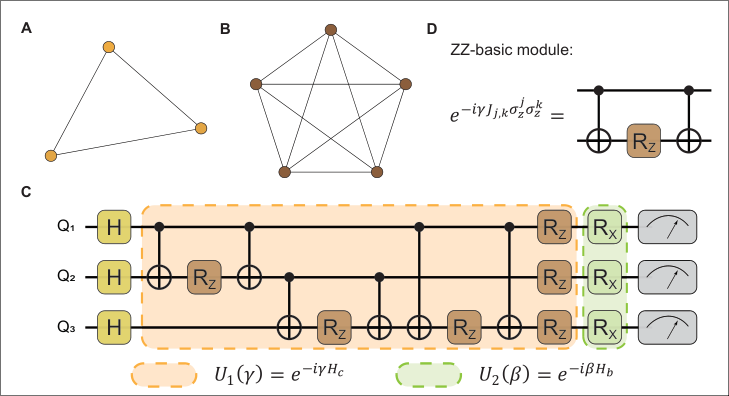
\includegraphics[scale=0.6]{inc/fig_11.png}
    \caption{
    Связность кубитов и типичная квантовая схема QAOA. A — топология связности
    кубитов для случая с 3 кубитами, представляющая собой граф $K_3$. B —
    случай с 5 кубитами, соответствующий графу $K_5$. C — типичная квантовая
    схема QAOA с одним слоем для гамильтониана QUBO на 3 кубитах. Она в
    основном состоит из двух операторов: $U_1(\gamma)$ и $U_2(\beta)$,
    соответствующих операторам эволюции проблемного гамильтониана $H_c$ и
    смешивающего гамильтониана $H_b$ соответственно. D — базовый модуль ZZ. Он
    состоит из двух CNOT-затворов и одного однокубитного вращения $R_z$,
    расположенных по схеме «бутерброда».
    }
    \label{fig:fig11}
\end{figure}

\subsection*{Глубина схемы при топологии полного графа}

Сначала рассмотрим идеальный случай, при котором любые два кубита могут
напрямую взаимодействовать. Иначе говоря, топология связности кубитов в
физической системе представляет собой полный граф. В этом сценарии задача
внедрения схемы типа $K_n$ не требует дополнительных кубитов или квантовых
SWAP-затворов. Следовательно, глубина квантовой схемы может быть
минимизирована.

Полный граф $K_n$ содержит $n(n - 1)/2$ рёбер, что означает, что схема QAOA
содержит $O(n^2)$ базовых модулей ZZ. Глубина однослойной схемы QAOA без
оптимизации составляет $O(n^2)$. Поскольку ZZ-члены в операторе $U_1(\gamma)$
коммутируют между собой, мы можем произвольно переставлять порядок двухкубитных
взаимодействий, чтобы минимизировать глубину схемы.

Здесь мы представляем схему оптимизации, основанную на теории максимального
паросочетания в неориентированном графе, которая позволяет уменьшить глубину
схемы до $O(n)$. Эта схема является оптимальной, если рассматривать ZZ-член как
базовый модуль.

\textbf{Определение 2}. Паросочетание и максимальное паросочетание. Обозначим
неориентированный граф как $G(V, E)$ и пусть $M \subseteq E(G)$ — подмножество
рёбер, такое что для всех пар $(e_i, e_j) \in M$ рёбра $e_i$ и $e_j$ не смежны
в $G$. То есть рёбра в $M$ не имеют общих вершин. Тогда $M$ называется
паросочетанием в графе $G$. Для каждого ребра $e = (u, v)$ в паросочетании $M$,
говорят, что ребро $e$ и вершины $u$, $v$ покрыты паросочетанием $M$. Каждая
вершина в графе либо не покрыта $M$, либо покрыта ровно одним ребром из $M$.
Если не существует другого паросочетания $M'$ в $G$, такого что $|M'| > |M|$,
то $M$ называется максимальным паросочетанием в $G$. Если каждая вершина в $G$
покрыта паросочетанием $M$, то $M$ называется совершенным паросочетанием в $G$.

Согласно определению, совершенное паросочетание обязательно является
максимальным. Количество максимальных паросочетаний в полном графе определяется
следующей леммой.

\textbf{Лемма 3} (Максимальное паросочетание в полном графе) Существует $2n -
1$ совершенных паросочетаний без повторяющихся рёбер в полном графе чётного
порядка $K_{2n}$. Аналогично, существует $2n - 1$ максимальных паросочетаний
без повторяющихся рёбер в полном графе нечётного порядка $K_{2n - 1}$.

\textit{Доказательство.} Для полного графа чётного порядка $K_{2n}$ расположим
вершины $v_1, v_2, \dots, v_{2n-1}$ по окружности в виде $(2n - 1)$‑угольника и
добавим вершину $v_{2n}$ в центр. Выберем произвольную вершину $v_i$, где $1
\leq i \leq 2n - 1$, и построим паросочетание $M_i$, включающее ребро $(v_i,
v_{2n})$ и все рёбра, перпендикулярные ему. Легко доказать, что $M_i$ —
совершенное паросочетание для любого $i$, и ни одно ребро не повторяется между
$M_i$ и $M_j$, если $i \ne j$. Таким образом, в полном графе $K_{2n}$
существует $2n - 1$ совершенных паросочетаний без повторений. Так как в графе
$K_{2n}$ всего $n(2n - 1)$ различных рёбер, и $2n - 1$ совершенных
паросочетаний уже покрывают их без повторений, других возможных неповторяющихся
паросочетаний не существует. Для случая нечётного полного графа $K_{2n - 1}$
добавим вспомогательную вершину $v_{2n}$, тем самым превратив задачу в случай
чётного порядка. Затем в каждом совершенном паросочетании удалим ребро $(v_i,
v_{2n})$. В результате получим $2n - 1$ максимальных паросочетаний для
нечётного случая. Это завершает доказательство.

\textbf{Утверждение 3}

Если связность кубитов в физической системе представляет собой полный граф, то
гамильтониан типа $K_n$ может быть внедрён без дополнительных кубитов, а
глубина внедрённой квантовой схемы составляет $O(n)$.

\textit{Доказательство.} Согласно определению паросочетания (см. Определение
2), рёбра в одном паросочетании не имеют общих вершин. Следовательно,
соответствующие двухкубитные взаимодействия можно выполнять одновременно и
параллельно. Предположим, что каждый ZZ-член компилируется с использованием
базового модуля ZZ (см. рис.~S7D), тогда глубина схемы для одного паросочетания
равна 3. Согласно Лемме 3, если $n$ чётно, то в полном графе $K_n$ существует
$n - 1$ неповторяющихся совершенных паросочетаний, покрывающих все рёбра.
Значит, можно построить квантовую схему из $n - 1$ слоёв, где каждый слой
содержит $n/2$ модулей ZZ, выполняемых параллельно. Общая глубина схемы
составит $3(n - 1)$. Если $n$ нечётно, то по Лемме 3 в полном графе $K_n$
существует $n$ максимальных паросочетаний без повторяющихся рёбер. Каждое такое
паросочетание содержит $(n - 1)/2$ рёбер, и все вместе они покрывают все рёбра
графа $K_n$. Значит, можно построить квантовую схему из $n$ слоёв, каждый из
которых выполняет $(n - 1)/2$ двухкубитных операций параллельно. Общая глубина
схемы составляет $3n$. Таким образом, схема типа $K_n$ может быть реализована
без дополнительных кубитов, а глубина внедрённой квантовой схемы составляет
$O(n)$. Доказательство завершено.

Доказательство Леммы 3 предоставляет точную конструкцию каждого совершенного
паросочетания в полном графе $K_n$, а значит — и точную схему построения
внедрённой квантовой схемы с глубиной $O(n)$. Схема оптимальна, если
рассматривать ZZ-члены в качестве базового модуля. В таком случае количество
ZZ-операций в каждом слое максимально, то есть достигается наивысшая степень
параллелизма. Поскольку все максимальные (совершенные) паросочетания покрывают
все рёбра без повторений, схема является оптимальной.

Связность кубитов — это ценный ресурс в устройствах NISQ. Как правило,
построение полносвязной топологии в масштабируемых квантовых системах
затруднено. Тем не менее, она достижима в некоторых особых системах, таких как
ионные ловушки~\cite{cite_52}, оптические квантовые системы и системы с большой
квантовой памятью~\cite{cite_15}.

\subsection*{Глубина схемы при линейной и решётчатой топологиях}

Линейная цепочка (linear chain) — одна из самых распространённых топологий,
которая относительно легко реализуется в реальных квантовых системах. Эта
топология, также известная как архитектура линейного ближайшего соседа (LNN),
предполагает расположение кубитов на линии с возможностью взаимодействия только
между соседними кубитами. В этом разделе мы рассматриваем ресурсы по числу
квантовых затворов и глубине схемы при внедрении гамильтониана типа $K_n$ в
одномерную систему LNN. Результаты для двумерной решётки (lattice system) можно
сформулировать как следствие.

Задача внедрения произвольных топологий гамильтонианов в LNN широко
исследуется~\cite{cite_53,cite_54,cite_55,cite_56,cite_57,cite_58,cite_59}, и
уже существуют зрелые методы. В 2007 году Донни Чеунг и др.~\cite{cite_55}
исследовали накладные расходы при преобразованиях между различными топологиями
на основе графовых моделей. Они указали, что отображение произвольной схемы в
LNN требует не более $O(n)$ дополнительной глубины на основе параллельной
сортировки. Однако конкретная схема преобразования гамильтониана типа $K_n$ в
LNN ими не приводится. В 2009 году Юити Хирата предложил эффективный метод
отображения произвольных квантовых схем в LNN на основе идеи пузырьковой
сортировки~\cite{cite_56}. В 2021 году исследователи из Google применили
параллельную пузырьковую сортировку для выполнения внедрения из $K_{17}$ в LNN
и провели соответствующие эксперименты на сверхпроводниковом квантовом
процессоре Sycamore~\cite{cite_11}. В целом, отображение $K_n$ в LNN требует
$O(n^2)$ операций SWAP и $O(n)$ дополнительной глубины схемы при использовании
параллельной пузырьковой сортировки. Ниже мы приведём независимое
доказательство этого результата на основе параллельного пузырькового алгоритма.

Чтобы внедрить полный граф $K_n$ в LNN, необходимо выполнять дополнительные
SWAP-операции для перестановки (или сортировки) кубитов в нужном порядке.
Минимизация числа SWAP-затворов является ключевой задачей. Согласно
работе~\cite{cite_56}, сеть SWAP-операций пузырьковой сортировки оптимальна для
этой цели. Следовательно, справедлива следующая лемма.

\textbf{Лемма 4.} Пусть $x_1, x_2, \dots, x_n$ — начальный порядок $n$ кубитов
в архитектуре LNN. Рассмотрим перестановку, изменяющую порядок на $x_{j_1},
x_{j_2}, \dots, x_{j_n}$. Минимальное число необходимых SWAP-затворов
эквивалентно числу операций обмена в алгоритме пузырьковой сортировки.

Лемма 4 показывает, что пузырьковая сортировка является оптимальной для
перестановки порядка кубитов в случае, когда возможно взаимодействие только
между соседними. Таким образом, квантовая схема SWAP-перестановок эквивалентна
классической пузырьковой сортировке.

Пузырьковая сортировка начинается с головы массива данных, сравнивает первые
два элемента и, если первый больше второго, меняет их местами. Процесс
повторяется для каждой пары соседних элементов, пока не будет достигнут конец
массива. Повторяется до тех пор, пока за один проход не произойдёт ни одной
перестановки. Каждая пара сравнивается только один раз, поэтому среднее и
худшее время выполнения составляет $O(n^2)$.

Рассмотрим худший случай: начальный порядок $1, 2, \dots, n$, и требуется
получить обратный порядок $n, n-1, \dots, 1$. Согласно лемме 4, пузырьковая
сортировка требует наименьшего числа SWAP-затворов. В этом случае необходимо
$n(n-1)/2$ обменов, что в точности покрывает все рёбра полного графа $K_n$.
Следовательно, классическая сеть пузырьковой сортировки, реализующая обратную
перестановку, эквивалентна внедрению гамильтониана типа $K_n$ в LNN.

Параллельная пузырьковая сортировка позволяет сократить время выполнения до
$O(n)$. Основная идея — одновременное сравнение всех соседних пар входных
данных с чередованием между нечётной и чётной фазами. Псевдокод приведён в
Алгоритме~4. При размере входных данных $n$ алгоритм выполняет $n$ итераций.
Каждая итерация делится на чётную и нечётную фазы в зависимости от номера шага.
Если $n$ нечётно, каждая фаза выполняет $(n - 1)/2$ операций сравнения и
обмена, которые можно проводить параллельно. Если $n$ чётно, то нечётная и
чётная фазы выполняют $n/2$ и $n/2 - 1$ операций соответственно.

\begin{algorithm}[htp!]
    \SetAlgoLined

    \KwData{Data, массив из $n$ элементов}
    \KwResult{Data в обратном порядке}

    \For{$i \gets 1$ \KwTo $n$}{
        Flag $\gets \mathrm{mod}(i, 2)$; \tcp*[r]{флаг для чётной и нечётной фазы}

        \For{$j \gets 1$ \KwTo $\left\lfloor \dfrac{n - 1 + \text{Flag}}{2} \right\rfloor$}{
            \If{$\text{Data}[2j - \text{Flag}] < \text{Data}[2j + 1 - \text{Flag}]$}{
                swap Data[$2j - \text{Flag}$] и Data[$2j + 1 - \text{Flag}$];
            }
        }
    }

    \caption{Параллельная пузырьковая сортировка}
    \label{alg:parallelBubble}
\end{algorithm}

Следующая лемма справедлива для алгоритма параллельной пузырьковой сортировки.

\textbf{Лемма 5.} Пусть $n$ — размер входных данных, а $p \leq \lfloor n/2
\rfloor$ — число доступных процессоров. Тогда временная сложность алгоритма
составляет $O(n^2 / 2p)$. Минимум достигается при $p = \lfloor n/2 \rfloor$ с
не более чем $n$ итерациями.

Если количество процессоров меньше $n/2$, то один процессор выполнит примерно
$\lfloor n / 2p \rfloor$ операций сравнения и обмена во внутреннем цикле каждой
фазы. В этом случае сложность алгоритма составляет $O(n^2 / 2p)$. При этом
оптимальное количество процессоров — $\lfloor n/2 \rfloor$, и каждый процессор
во внутреннем цикле выполняет не более одной операции. Внешний цикл алгоритма
завершит всю пузырьковую сортировку за не более чем $n$ итераций. В квантовых
вычислениях предполагается, что устройство обладает достаточным числом
управляющих процессоров, чтобы выполнять двухкубитные операции параллельно,
если они не используют один и тот же кубит. Отсюда следует следующий результат.

\textbf{Утверждение 4.} Схема типа $K_n$ может быть внедрена в физическую
систему с топологией LNN без дополнительных кубитов, и глубина внедрённой
квантовой схемы составляет $O(n)$.

\textit{Доказательство.} Пусть начальный порядок кубитов в системе LNN: $1, 2,
\dots, n$, и он перестраивается в обратный порядок: $n, n-1, \dots, 1$.
Пузырьковая сортировка требует $n(n-1)/2$ перестановок. Сеть обменов
пузырьковой сортировки точно покрывает все рёбра полного графа $K_n$, тем самым
реализуя внедрение схемы $K_n$ в LNN. Этот процесс реализуется параллельной
пузырьковой схемой $\Gamma$ с $n/2$ процессорами. Согласно лемме 5, схема
требует не более $n$ итераций, и на каждой итерации выполняется $\lfloor n/2
\rfloor$ обменов параллельно. Конкретная параллельная сеть SWAP-операций,
реализующая данный процесс, показана на рис. \ref{fig:fig12}. Следовательно,
внедрённую схему в системе LNN можно построить, заменив SWAP-затвор в $\Gamma$
на базовый модуль ZZ-SWAP (см. рис.~S8C). Так как глубина модуля ZZ-SWAP
составляет 4, то общая глубина схемы — $4n$. Весь процесс внедрения не требует
дополнительных кубитов. Доказательство завершено.

\begin{figure}
    \centering
    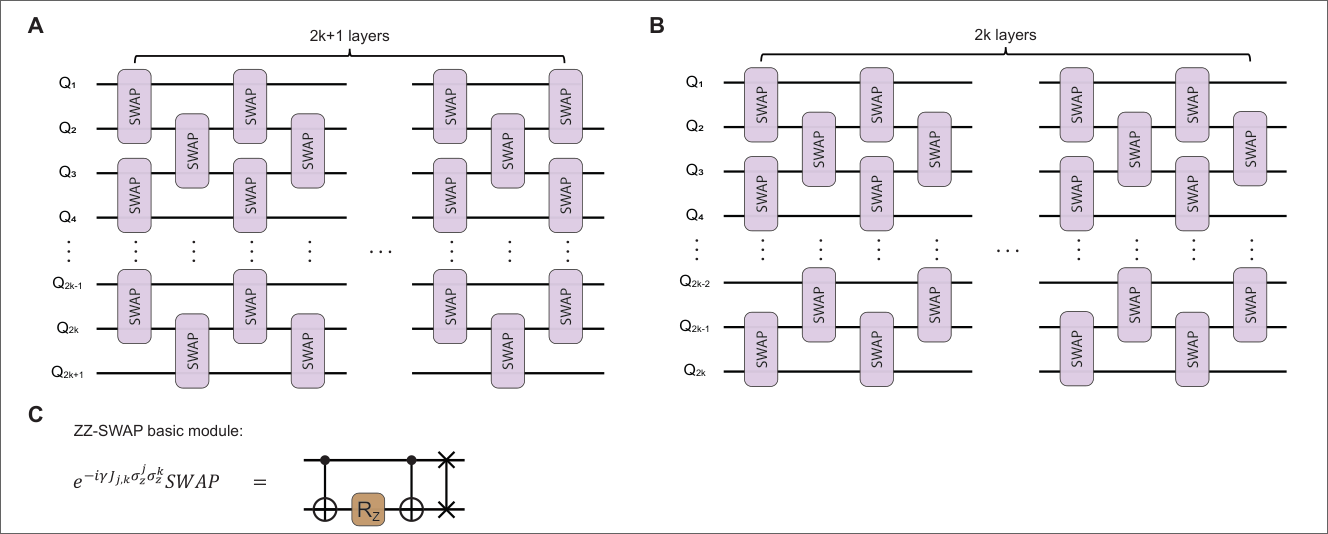
\includegraphics[scale=0.35]{inc/fig_12.png}
    \caption{
    Схема параллельной пузырьковой сортировки, реализующей обратную
    перестановку. A — случай нечётного числа кубитов, B — случай чётного числа
    кубитов. В обоих случаях количество слоёв внешнего цикла составляет $n$,
    что приводит к глубине схемы $O(n)$. C — базовый модуль ZZ-SWAP: это
    квантовая схема глубины 4, представляющая собой операцию SWAP, выполненную
    после базового модуля ZZ.
    }
    \label{fig:fig12}
\end{figure}

Кроме того, поскольку каждый ZZ-член в $K_n$ становится модулем ZZ-SWAP,
требуется дополнительная нагрузка в виде $n(n-1)/2$ операций SWAP и глубины $n$
после внедрения. После выполнения схемы порядок кубитов окажется обратным, и
его можно восстановить, снова запустив схему QAOA.

Система с решётчатой топологией (lattice topology) также известна как двумерная
квадратная решётка (2DSL), в которой кубиты располагаются в виде двумерной
решётки, и разрешены только соседние взаимодействия. Поскольку одномерная
цепочка может быть непосредственно вложена в двумерную решётку (например, вдоль
одной из диагоналей или рядов), глубина внедрённой схемы для гамильтониана типа
$K_n$ не будет превышать глубину в случае LNN. Следовательно, справедливо
следующее следствие.

\textbf{Следствие 1.} Глубина схемы для гамильтониана типа $K_n$, внедрённой в
двумерную квадратную решётку (2DSL), составляет $O(n)$ и не требует
дополнительных кубитов.

Полная топология графа является идеальной топологией: схема гамильтониана типа
$K_n$ может быть внедрена оптимально по глубине $O(n)$ без каких-либо
дополнительных квантовых ресурсов. Для топологии LNN необходима дополнительная
глубина $O(n)$. Поскольку схема внедрения на основе параллельной пузырьковой
сортировки также имеет сложность $O(n)$, она является оптимальной как для LNN,
так и для 2DSL-систем в смысле нотации $\mathcal{O}$. Кроме того, в
работе~\cite{cite_55} предложен более эффективный метод внедрения гамильтониана
типа $K_n$ в систему 2DSL с дополнительной глубиной $O(\sqrt{n})$, что
достигается за счёт удобной двумерной структуры.

\subsection*{Оценка ресурсов для факторизации RSA-2048}

В этом разделе мы обсуждаем необходимые квантовые ресурсы для атаки на реальные
RSA-числа на основе полученных выше результатов. Поскольку внедрение схемы не
требует дополнительных кубитов, количество кубитов, необходимое для
факторизации $m$-битного числа, оценивается как $n = \frac{2m}{\log m}$ (здесь
параметр точности $c = 1$). Глубина внедрённой схемы для гамильтониана типа
$K_n$ составляет $3n$ для полностью связанной системы, $4n$ — для системы с
линейной топологией (LNN) и $3n + \sqrt{n}$ — для двумерной решётки (2DSL),
согласно Donny Cheung и соавт.~\cite{cite_55}. Эти оценки получены без учёта
особенностей компиляции базового модуля ZZ (или ZZ-SWAP) в конкретной
физической реализации. В качестве примера рассмотрим RSA-2048. Число кубитов:
$\frac{2 \cdot 2048}{\log 2048} \approx 372$. Глубина схемы однослойного
алгоритма QAOA составляет приблизительно $3n + 2 = 1118$ в полностью связанной
системе, где 2 дополнительных уровня приходятся на однокубитные операции: один
уровень для $R_z$-вращений и один — для $R_x$-вращений. а для двумерной
квадратной решётки (2DSL) — около $3n + \sqrt{n} + 2 = 1139$. Необходимые
квантовые ресурсы для факторизации RSA-чисел различной длины приведены в
Таблице З.10.

\begin{table}[H]
\centering
\caption{
    Оценка квантовых ресурсов для RSA-чисел. Основные квантовые ресурсы,
    рассматриваемые здесь, — это количество кубитов и глубина квантовой схемы
    однослойного алгоритма QAOA в трёх типичных топологиях: полностью связанной
    системе ($K_n$), двумерной решётке (2DSL) и одномерной цепочке (LNN).
    Полученные результаты не учитывают особенности компиляции базового модуля
    ZZ (или модуля ZZ-SWAP) в конкретной физической реализации.
}
\begin{tabular}{c|c|c|c|c}
\hline
\hline
\textbf{RSA } & \textbf{Кубиты} & \textbf{Kn глубина} & \textbf{2DSL глубина} & \textbf{LNN глубина} \\
\hline
RSA-128  &  37  & 113  & 121  & 150 \\
RSA-256  &  64  & 194  & 204  & 258 \\
RSA-512  & 114  & 344  & 357  & 458 \\
RSA-1024 & 205  & 617  & 633  & 822 \\
RSA-2048 & 372  & 1118 & 1139 & 1490 \\
\hline
\hline
\end{tabular}
\end{table}

Мы также проанализировали масштаб RSA-чисел, а именно предельный размер
(touch-size), которого могут достичь современные квантовые вычислительные
устройства при некоторых идеальных условиях, при которых все заявленные кубиты
считаются относительно идеальными или обладающими высокой достоверностью.
Результаты приведены в соответствии с топологией связности кубитов квантовых
устройств с использованием алгоритма SQIF. Рассматриваемые квантовые процессоры
включают: Sycamore, Eagle, Aspen-M, Zuchongzhi2, Tianmu-1, а также ионные
ловушки, разработанные в Мэриленде и компанией IonQ. Все эти устройства либо
находятся в публичном доступе, либо доступны через облачные квантовые
платформы. Кроме того, мы указываем минимальную необходимую глубину схемы
(``depth-least'') для этих устройств, при которой можно попытаться
факторизовать RSA-числа предельного размера. Эта глубина оценивается по глубине
однослойной схемы QAOA.В частности, если квантовый процессор имеет двумерную
решётчатую топологию, глубина схемы рассчитывается по модели 2DSL. Для
топологий типа ``прочие'' глубина рассчитывается по модели LNN. Подробные
результаты приведены в Таблице З.11.

Из Таблицы З.11 видно, что предельный размер для устройств NISQ уже близок к
реальным RSA-числам. Например, 127-кубитная машина \texttt{ibm-eagle} имеет
предельный размер 581, а минимально необходимая глубина схемы составляет 510.
Это означает, что если все кубиты функционируют стабильно и обеспечивают
достаточную точность после 510 уровней схемы, устройство может быть
использовано для попытки факторизации RSA-581.

Тем не менее, предельный размер — это идеализированная оценка. На практике
алгоритм QAOA обычно требует более чем одного слоя, что увеличивает глубину
схемы. Кроме того, наличие квантового ускорения по-прежнему остаётся
неизвестным, и квантовый взлом RSA пока остаётся далёкой целью.

\begin{table}[ht]
\centering
\caption{
    Предельный размер RSA-чисел для некоторых известных квантовых устройств.
    Результаты приведены на основе топологии связности кубитов и набора базовых
    логических затворов соответствующих квантовых устройств, с использованием
    предложенного нами алгоритма. Последний столбец указывает минимальное
    условие по глубине схемы, которое должно быть выполнено для возможности
    факторизации. Для систем с топологией типа ``прочие'' глубина схемы
    рассчитывается по модели LNN.
    }
\resizebox{\textwidth}{!}{%
\begin{tabular}{|c|c|c|c|c|c|}
\hline
\textbf{Система} & \textbf{Устройство} & \textbf{Кубиты} & \textbf{Топология} & \textbf{Предельный размер} & \textbf{Мин. глубина} \\
\hline
\multirow{4}{*}{Сверхпроводящие кубиты}
& Sycamore      & 53  & 2DSL   & 201 & 170 \\
& Eagle         & 127 & прочие & 581 & 510 \\
& Aspen-M       & 80  & прочие & 334 & 322 \\
& Zuchongzhi2   & 66  & 2DSL   & 264 & 210 \\
& Tianmu-1      & 36  & 2DSL   & 124 & 118 \\
\hline
\multirow{2}{*}{Ионные ловушки}
& Maryland      & 40  & $K_n$  & 142 & 122 \\
& IonQ          & 79  & $K_n$  & 329 & 239 \\
\hline
\end{tabular}
}
\label{tab:device_resources}
\end{table}
